\documentclass[12pt,english]{article}
\usepackage{amsmath} % for equations
% for bibliographies 
\usepackage[round]{natbib} 
\setcitestyle{aysep={,},yysep={,},citesep={;},notesep={: }}
\usepackage[hidelinks]{hyperref}
\urlstyle{same}
% for tables and figures
\renewcommand{\thetable}{\Roman{table}}
\usepackage{caption}\captionsetup{labelsep = period}
\usepackage{graphicx}

% information for title page
\title{Tables and figures for ``An example Journal of Peace Research paper typeset in \LaTeX''}
\author{Name of Author \\ University of Author \\ Word count: 9000}


\begin{document}

%%%%%%%%%%%%%%%%%%%%%%
% Title Page

\maketitle

\newpage

%%%%%%%%%%%%%%%%%%%%%%
% Tables

\begin{table}[h!]
\caption{An example of a table}
\centering
\begin{tabular}{||c c c c||} 
 \hline
 Col1 & Col2 & Col2 & Col3 \\ [0.5ex] 
 \hline\hline
 1 & 6 & 87837 & 787 \\ 
 2 & 7 & 78 & 5415 \\
 3 & 545 & 778 & 7507 \\
 4 & 545 & 18744 & 7560 \\
 5 & 88 & 788 & 6344 \\ [1ex] 
 \hline
\end{tabular}
\label{table:1}
\end{table}

%%%%%%%%%%%%%%%%%%%%%%
% Figures

\begin{figure}[hbtp]
\caption{An example of a figure}
\centering
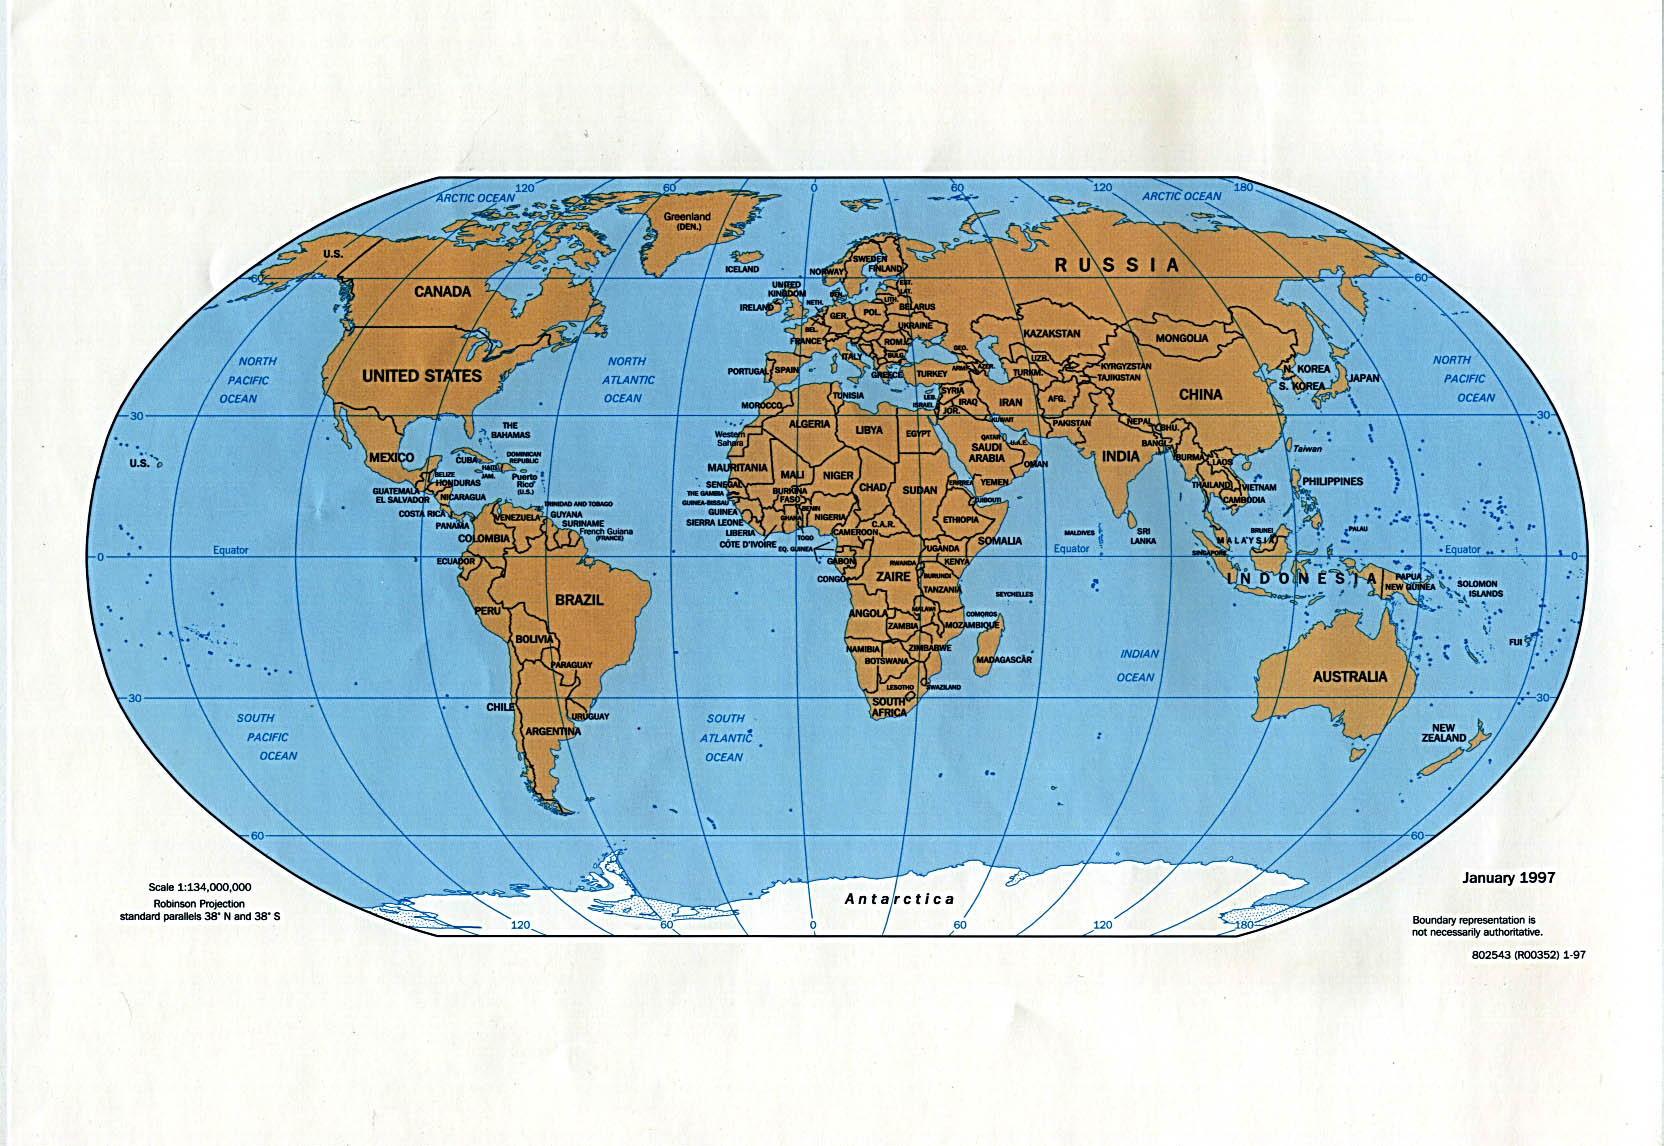
\includegraphics[scale=0.3]{world_map.jpg}
\end{figure}




\end{document}
